%%%%%%%%%%%%%%%%%%%%%%%%%%%%%%%%%%%%%%%%%%%%%%%%%%%%%%%%%%%%%%%%%%%%%%%%
%                                                                      %
%     File: Thesis_Results.tex                                         %
%     Tex Master: Thesis.tex                                           %
%                                                                      %
%     Author: Andre C. Marta                                           %
%     Last modified :  2 Jul 2015                                      %
%                                                                      %
%%%%%%%%%%%%%%%%%%%%%%%%%%%%%%%%%%%%%%%%%%%%%%%%%%%%%%%%%%%%%%%%%%%%%%%%

\chapter{Application to Deep Learning}
\label{chapter:results}

From the set of applications that are known to be imprecision tolerant, deep learning stands out as one of the most prominent ones. This chapter starts by providing a brief  overview about deep learning applications, presenting the concept of deep neural networks (\acrshort{dnn}), how the training of these algorithms is performed and how they are implemented using high-level libraries.

The chapter continues by applying non-conventional V-F scaling to the most energy consumption layers of a Convolutional Neural Network (\acrshort{cnn})~\cite{li_evaluating_2016}. Finally, the devised V-F Optimization Mechanism, described in Chapter~\ref{chapter:mech}, is applied to the training process of a \acrshort{cnn}, allowing the reduction of the consumed energy and massive a improvement on energy efficiency of \acrshort{gpu}s running this kind of algorithm.


%%%%%%%%%%%%%%%%%%%%%%%%%%%%%%%%%%%%%%%%%%%%%%%%%%%%%%%%%%%%%%%%%%%%%%%%
\section{Deep Learning Overview}
\label{section:problem}

In the last few years, Deep Learning (\acrshort{dl}), and more particularly Deep Neural Networks (\acrshort{dnn}), have had a significant impact in industry and society, by allowing for important breakthroughs in many application domains, such as computer vision, speech recognition, natural language processing, drug discovery, genomics, and others \cite{shrestha_review_2019}.

Deep Learning is a subset of the larger family of Machine Learning methods, also known as deep structured learning or hierarchical learning. This type of algorithms can be utilized for supervised, semi-supervised, and unsupervised learning \cite{bengio_representation_2013, schmidhuber_deep_2015}. Different Deep Learning architectures are being developed, such as convolutional neural networks (\acrshort{cnn}), recurrent neural networks (\acrshort{rnn}), and unsupervised pre-trained networks (\acrshort{upt}), targetting different objectives and being able to analyze and learn from the data in different ways. The general trend over the years is to increase the number of trainable parameters, usually denoted as weights of the network, to achieve better results. Such an increase in the tunable parameters not only demands an improvement in the device's memory - to accommodate the increased size of the model; in the device's performance - to be able to train and use the model in usable time; and more importantly, energy efficiency - to allow a sustained increase of the number of devices in supercomputers and to be able to run the algorithms in portable computing devices.

\subsection{Deep Neural Networks}

The central element of a deep neural network (DNN) is the artificial neuron. This element can be mathematically modeled by a set of multiplications and summations, as shown in Equation \ref{eq:neuron}, where $W_i$ represents the weight and $b$ is the bias applied on each artificial neuron.

\begin{equation}
\label{eq:neuron}
    Y = \sum_{i=1}^{n} W_iX_i+b
\end{equation}

One of the most significant benefits of deep neural networks is their ability to capture non-linear relationships between the input parameters. For such purpose, an activation function is usually attached to each neuron, helping him to handle scenarios where problems are not linearly separated \cite{dong_dnnmark:_2017}. The most common non-linear activation functions are hyperbolic tangent ($tanh$) \cite{orr_neural_1998}, Rectified Linear Unit (ReLU) \cite{orr_neural_1998} and sigmoid \cite{orr_neural_1998}. Hence, the prevailing deep neural network architecture is the combination of the linear transformations performed by the neurons plus the non-linear activation functions.

A neural network is an arrangement of neurons and activation functions in several layers. Each layer is responsible for applying a series of transformations to the data according to the weight and bias stored in each artificial neuron. As represented in Figure~\ref{fig:DNNarch}, a \acrshort{dnn} is composed of at least three layers, the input layer, with a number of neurons equal to the input size, at least one hidden layer, being this the distinguishing characteristics of a  \acrshort{dnn}, and an output layer with the number of neurons equal to the output size. The possible different organization of the layers in size, type of operation and number of connections of layers defines the type and architecture of the  \acrshort{dnn}.

\begin{figure}[!htb]
  \centering
  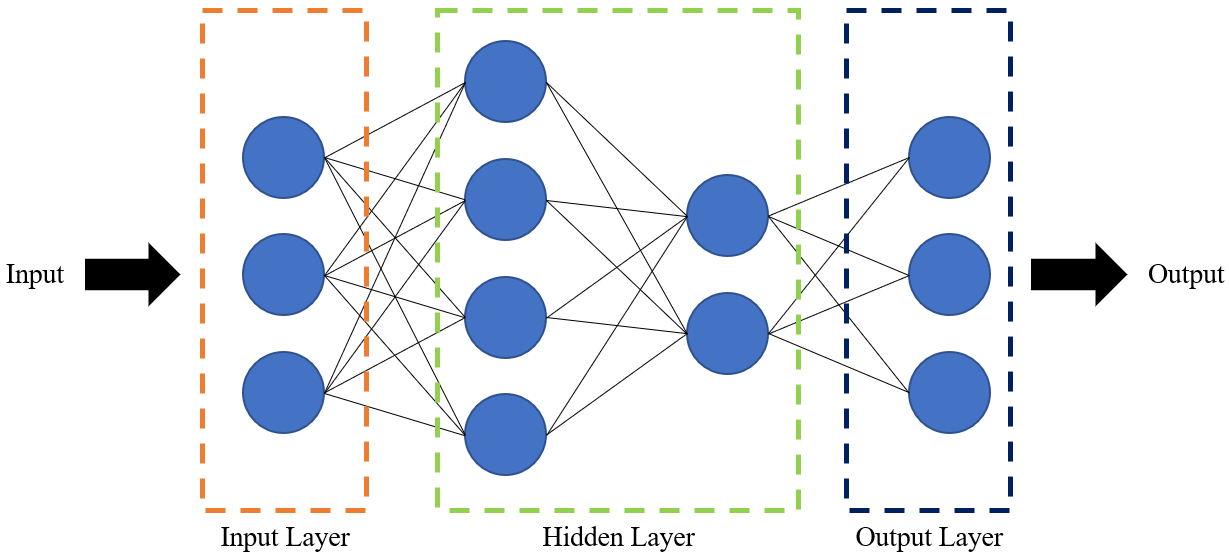
\includegraphics[width=0.6\textwidth]{Figures/Application To Deep Learning/DNNarch.png}
  \caption{Model of fully-connected (feed-forward) \acrshort{dnn}}
  \label{fig:DNNarch}
\end{figure}

\subsection{DNN Architectures}

Current \acrshort{dnn} architectures are grouped into three types of architecture, depending on the fundamental primitive operation being performed. These are Convolutional Neural Networks (\acrshort{cnn}), Recurrent Neural Networks (\acrshort{rnn}) and Unsupervised Pretrained Networks (\acrshort{upt}). 

\subsubsection{Convolutional Neural Networks (CNN)}
Convolutional Neural Networks are usually used to extract features from data via the convolution operation, being mainly used for image and object recognition and sound analysis. This type of architecture excels when there is some structure in the input data, that is, the data contains sets of specific patterns, organized in a spatial manner, that the neural network can learn to recognize.

The \acrshort{cnn} architecture generally follows the following pattern: input layer, feature-extraction layers and classification layer. The input layer receives a form of three-dimensional data, usually an image with a specific height and width and a depth value (representing color or intensity). The feature extraction layers perform higher-order features extract from the input, generally by performing patterns of convolution layers and pooling layers. Finally, the classification layer is a vector of size \textit{N}, where each output represents a score of prediction confidence for the input to be of a given output class.

Three common datasets that are often used to compare and analyse the \acrshort{cnn}  performance are MNIST~\cite{lecun_yann_and_cortes_corinna_mnist_1999}, CIFAR 10~\cite{krizhevsky_learning_2009} and ImageNet~\cite{deng_imagenet_2009}, each with increased input complexity, number of output classes and overall dataset size. MNIST consists of 70 000 images of handwritten digits 0 to 9, CIFAR10 consists of 60 000 organized images of 10 object and animal classes, and ImageNet is a collection of 14 million images of 20 thousand different classes. 

\subsubsection{Recurrent Neural Networks (RNN)}

Recurrent Neural Networks have the added capability of sending information over time-steps. This characteristic allows this type of architecture to have parallel and sequential data modeling, not only recognizing features from each input but also allowing for the extraction of features from the sequences of inputs, modeling the time dimension. 

\acrshort{rnn}s are often used to model time-series, language, audio, and text since this type of data is inherently ordered and context-sensitive. \acrshort{rnn}s contain feedback loops between the layers, allowing each layer to have insights about what happened before. The prediction model follows the general format presented in Equation \ref{eq:rnn}, where the current timestamp model output $y^{(t)}$ is a function $f$ of the previous models output $y^{(t-1)}$ and current model input $x^{(t)}$, in addition to a bias factor $\theta$. The equation reflects the influence of previous inputs for each output.
\begin{equation}
    \label{eq:rnn}
    %y[n] = x[n] + ... + x[n-i]
    y^{(t)}=f(y^{(t-1)}, x^{(t)}, \theta)
\end{equation}

The component responsible for the feature extraction characteristic of \acrshort{rnn} models is the LSTM - Long Short Term Memory. This type of layer has three gates - input, output and forget gates. The content of each LSTM is mainly defined by the input and forget gates; any change on these elements reflects on the value stored at the memory cell. If both gates are closed, the memory content remains unmodified between the current time-step and the following. Hence, the LSTM structure allows for information to be retained/forgotten on the memory cell across different time-steps.


\subsubsection{Unsupervised Pre-trained Networks (UPN)}
Unsupervised Pretrained Networks is a category of \acrshort{dnn} architectures that encompasses network structures such as autoencoders and generative adversarial networks (\acrshort{gan}s). This class of \acrshort{dnn} architecture contrasts with the previous ones by learning in an unsupervised manner, meaning that the input data given to the network is not previously labeled. This introduces an extra degree of learning freedom by allowing the network to identify and recognize patterns that distinguish the output classes the most.

Autoencoders are used to efficiently learn data codings and can be applied for dimensionality reduction or augmentation. Autoencoders provide a reduction of noise present in a signal or to perform a resolution increase on an image. \acrshort{gan}s can be used to perform sound and video synthesis from images or text using two neural networks in parallel - a discriminator and a generative network. First, the generative network creates a synthesized output from the given input. Then, the discriminator network tries to classify the input as real or synthesized, providing the classification to the generative network. With this data loop, the generative network updates their weights to fit best what is described as real data.


\subsection{Training and Inference}

The mathematical description of the \acrshort{dnn} training process, represented in Equation \ref{eq:loss}, is equivalent to treating the network as a loss function $L$, where inputs $X$, outputs $Y$ and the network's weights $W$ and bias $b$ are function arguments. The training session's objective is to optimize the in-network parameters  $W$ (weights) and $b$ (bias) to minimize the overall loss~\cite{rumelhart_learning_1986-1}.

\begin{equation}
    \label{eq:loss}
    (W,b) = \arg\min_{W} L(X,Y,W,b)
\end{equation}

The \acrshort{dnn} training is an iterative process, where at the end of each iteration, a loss value is computed, and the set of in-network parameters is updated. This loss value represents how well are the input parameters being modeled by the network. As the number of training iterations increases, the loss value reduces and converges to a minimum, at which the model prediction accuracy will be at its maximum. At this point, the training session can be stopped.

The most common method for the parameters update is the Stochastic Gradient Descent (\acrshort{sgd}) algorithm (see Equation \ref{eq:update}), an iterative algorithm that, after processing mini-batches of the training data, computes new weights and bias for each neuron~\cite{ruder_overview_2017}. 

\begin{equation}
    \label{eq:update}
    W_{i+1} \xleftarrow{} W_i - \alpha \sum_{n=1}^{m}\frac{\partial L}{\partial W_i}
\end{equation}

In Equation \ref{eq:update}, $m$ represents the number of mini-batches to run, $W_i$ is the current parameter, $W_{i+1}$ is the update parameter, $\alpha$ is the learning rate and $\frac{\partial L}{\partial W_i}$ is the partial derivative of the loss function $L$ in order to the parameters. This last equation is obtained by applying the derivative chain rule in a backward-cascade fashion with respect to inputs, outputs, and parameters of each \acrshort{dnn} layer.

Each iteration of the training process is composed of a forward and backward data propagation. On the forward propagation, the loss function for the current in-network parameters is evaluated, computing the loss value. By performing the backward propagation, the partial derivative $\frac{\partial L}{\partial W_i}$ of each of the parameters is obtained to apply the \acrshort{dnn} algorithm . 

Hence, the inference (or prediction) process corresponds to the execution of a forward propagation, with the intended input, on a previously trained neural network. At the output layer, a set of values (or probabilities) is computed, corresponding to the model's prediction to the given inputs.

\subsection{High-Level Libraries and Software Frameworks}

The popularization of \acrshort{gpu}s as the defacto \acrshort{dnn}s execution device results in the availability of high-level libraries and frameworks from device manufacturers and other software houses. The available \acrshort{gpu} libraries implement the underlying mathematical operations performed during the \acrshort{dnn}s, while the frameworks operate on the execution of \acrshort{dnn}s by masking the complexity of creating, training and using these models~\cite{jain_performance_2019}.

The most used libraries are cuBLAS\footnote{developer.nvidia.com/cublas} and cuDNN\footnote{developer.nvidia.com/cudnn}, by NVIDIA and rocBLAS\footnote{github.com/ROCmSoftwarePlatform/rocBLAS} and MIOpen\footnote{github.com/ROCmSoftwarePlatform/MIOpen}, by AMD, which implements the most optimized versions of matrix multiplication, convolution, and other mathematical operations to be used on the \acrshort{dnn} models. In what concerns the frameworks, TensorFlow\footnote{tensorflow.org/} and PyTorch\footnote{pytorch.org/} are open-source frameworks developed by Google and Facebook, respectively, that allow an easy implementation of the models in \acrshort{gpu}s.

%%%%%%%%%%%%%%%%%%%%%%%%%%%%%%%%%%%%%%%%%%%%%%%%%%%%%%%%%%%%%%%%%%%%%%%%
\section{DNN Performance and Energy Efficiency Improvement}
\label{section:DNN_conventional}

\acrshort{dnn}s are usually characterized by significant computational burdens, particularly when considering the training of very deep and complex networks that deal with high dimensional data, such as images and videos. For such purpose, researchers (and data scientists, in general) often rely on accelerators, such as \acrshort{gpu}s, to cope with the associated computational burden and reduce the training time. As a result, \acrshort{gpu}s are now commonly deployed on most supercomputers, data centers and other computational infrastructures related to the development of artificial intelligence algorithms.

Additionally, several software frameworks, algorithms and techniques have been proposed to manage and optimize the execution of  \acrshort{dnn}s on \acrshort{gpu}s (e.g., Mittal~\cite{mittal_survey_2019}). However, most optimization techniques neglect the training phase's energy impact, usually resulting in considerable costs. 

To overcome this problem, researchers have also explored other solutions that allow mitigating the energy impact of neural network training. One particular and common approach relies on the use of low-precision arithmetic (e.g., Nabavinejad~\cite{nabavinejad_coordinated_2019}), eventually trading network accuracy with increased processing performance and lower energy consumption.

Researchers have also looked at alternative approaches, such as exploiting \acrshort{dvfs} on both the inference and training phases. In fact, by carefully selecting the used voltage-frequency (V-F) levels, significant energy savings can be obtained, although depending on the considered \acrshort{dnn} architecture and computing  device~\cite{tang_impact_2019}. This is achieved by a careful balance between the performance and power consumption of the different \acrshort{gpu} components  (particularly the core and global memory) to minimize the stalls in the compute cores. In fact, not only can \acrshort{dvfs} be used to decrease the power consumption, but it can also boost the system performance~\cite{tang_impact_2019}, by increasing the voltage and frequency levels (as long as the GPU total power envelope and thermal limits are not surpassed).

%Nevertheless, as discussed, most state-of-the-art works only consider tightly coupled V-F levels, which are often predefined by GPU manufacturers and neglect the voltage margin that is usually introduced to guarantee fail-safe designs well as its variation with the kernel instruction sequence and the corresponding use of specific \acrshort{gpu} components. 


Hence, supported on the performed \acrshort{gpu} characterization to non-conventional V-F pairs, this work continues by exploring the impact of these configurations on \acrshort{cnn} layers, considering both the training and inference phases.

%%%%%%%%%%%%%%%%%%%%%%%%%%%%%%%%%%%%%%%%%%%%%%%%%%%%%%%%%%%%%%%%%%%%%%%%
\section{Non-conventional V-F on CNNs}
\label{section:baseline}

As it was referred in Section~\ref{sec:under_int_app}, Tang~\cite{tang_impact_2019} has recently studied the impact of frequency scaling on the performance and energy consumption of \acrshort{dnn}s executed in \acrshort{gpu}s. By extending this study with the capability to also apply undervoltage techniques, a broader range of \acrshort{dvfs} configurations are herein envisaged to provide even greater benefits. 

Another important characteristic of \acrshort{dnn}s is their tolerance to a certain degree of computation errors \cite{zhang_approxann_2015}, without any significant change in the training and inference results. Consequently, it is important to complement the characterization that was performed in Chapter~\ref{chapter:gpu_char} with the voltage scaling effects in \acrshort{dnn} training and inference phases and, in particular, with its influence on the computation errors that might occur when exploring the existing voltage margins.

As discussed before, at the particular case of the \acrshort{cnn}, its feature extraction ability is mostly supported by the convolution operator. Nonetheless, \acrshort{cnn} also includes other types of layers, such as fully connected and pooling layers. However, the convolution and fully connected layers take up to $97\%$ of the \acrshort{gpu} energy consumption~\cite{li_evaluating_2016}, which makes them particularly suited to exploit energy-saving mechanisms. 

Hence, to apply and assess non-conventional V-F pairs on the execution of \acrshort{cnn}s, the high-level deep learning framework PyTorch and the default mathematical libraries (rocBLAS and MIOpen) provided by the considered \acrshort{gpu} manufacturer (AMD) were extensively evaluated on the Vega 10 \acrshort{gpu}. This section reports the main achieved conclusions for the convolution operator and fully connected layers.

\subsection{Convolution Layer}

The AMD MIOpen library provides multiple convolution implementations, being the \textit{Direct}, \textit{GEMM} and \textit{Winograd}~\cite{khan_miopen_2019} the ones that are more often used. 
At the beginning of the execution, this library performs one convolution operation with each of the algorithms that are able to solve the required operation. Then, the algorithm that takes the shortest execution time is chosen and used to perform the remaining convolutions of the current layer. The convolution layer is defined by the parameters presented in Table~\ref{tab:convparams}. 

\begin{table}[htbp]
\begin{center}
\begin{tabular}{cl}
\hline
\textbf{Parameter}&\textbf{Description} \\ 
\hline
W, H & Input Width, Height\\
N & Mini-batch Size \\
C, K & Number of features, kernels \\
R, S & Kernel Width,Height\\
Pad\_W, Pad\_H & Padding Width, Height \\
Str\_W, Str\_H & Stride Width, Height \\
\hline
\end{tabular}
\label{tab:convparams}
\end{center}

\caption{Convolution Parameters.}
\end{table}

At this respect, a relevant question that may be raised is about the existance of a convolution algorithm that is more energy-efficient than the others. Such question is of particular interest for this work. If such possibility is there, it can be exploited by using one of the input parameters of the convolution \acrshort{api} that allows the algorithm selection, disabling the automatic algorithm selection procedure. 
To answer to such question, the execution time, and energy and power consumption of all algorithms were measured while executing 100 different convolutions layer configurations from the DeepBench benchmark\footnote{github.com/baidu-research/DeepBench}, with each algorithm being executed ten times with the median results being taken. The obtained results showed that the algorithm that achieved the shortest execution time in all cases also achieved the best energy consumption. By looking at the power consumption across the different algorithms, the result showed that it was similar in all cases. Two other important results were that no algorithm proved to be the fastest for all or for any subset of configurations and 
that not all convolution layer configurations are able to be 
solved by all 
%mapped on the pre-compiled and optimized kernels, that implement 
the different algorithms available in the library. 
As previously explained, the library executes one convolution using each available algorithm to determine which are able to solve it to compare the execution time between the different alternatives, choosing the one with the shorter execution time. Even though this technique appears simplistic and with space to be further optimized, the results show that, in reality, that is not the case. Measuring the execution time at the beginning of the execution for all possible execution alternatives optimizes both the performance as well as energy consumption since power consumption is similar between all the different convolution algorithms. This technique also brings the benefit of optimizing the execution to the current \acrshort{gpu} state and utilization, which is one of the premisses of the presented work.

To conduct this convolution analysis, a set of 20 distinct convolution layer configurations was selected from the DeepBench benchmark to understand how each algorithm is affected by the V-F configuration, both in its inference and training phases.



\subsubsection{Layer Guardband and Characterization}

Figure~\ref{fig:Convolution_guardband} presents the set of valid voltage ranges that were obtained for the inference and training phases of the convolution layer. By comparing these results with those obtained in the individual component characterization, it can be observed that some computation errors (and even some \acrshort{gpu} crashes) were detected at lower frequencies. In fact, since this operation is more complex and requires the utilization of multiple architectural components, the undervoltage limit is more likely to be violated by the voltage drops induced by the activation and deactivation of the \acrshort{gpu}  architectural components \cite{thomas_core_2016}. This phenomenon will make certain parts of the \acrshort{gpu} not to work properly (even momentarily), producing an increased rate of computation errors and an increased crash threshold voltage. 


\begin{figure}[htbp]
    \centering
        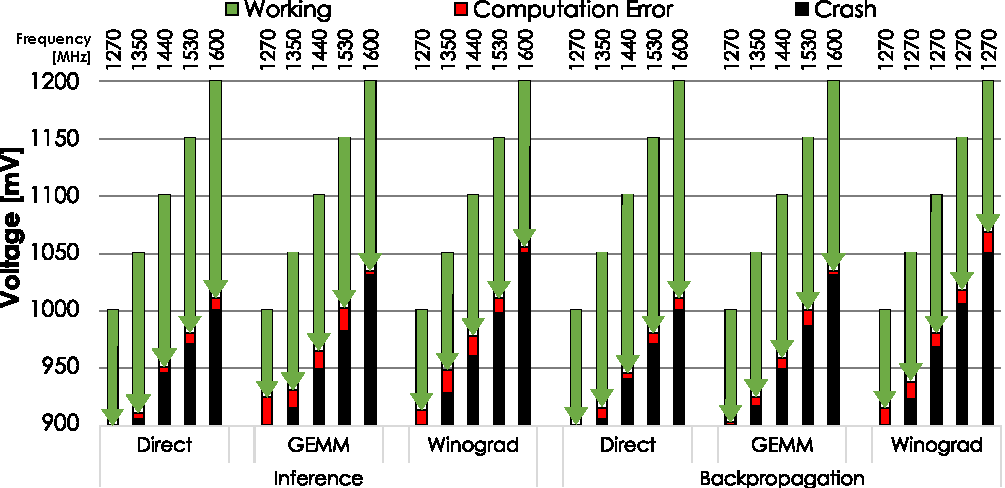
\includegraphics[width=0.75\textwidth]{Figures/Application To Deep Learning/Convolution_Guardband.pdf}
        \caption{Core Domain - Convolution Layer - Usable voltage range.}
    \label{fig:Convolution_guardband}
\end{figure}

When comparing the three convolution algorithms, it is observed that the \textit{Direct} algorithm allows for the greatest amount of undervoltage, followed by \textit{GEMM} and \textit{Winograd}. The \textit{Direct} algorithm is the simpler of the three, with no data transformation and movement being necessary for its execution. In contrast, \textit{GEMM} and \textit{Winograd} need some data pre-processing before the convolution is performed. This extra step relies on the activation of more \acrshort{gpu} components, making these algorithms more prone to induce voltage drops. 

When comparing the training and inference phases, it is observed that they present similar undervoltage capabilities (for all algorithms), with the crash point diverging only around $10$mV. However, the training algorithm is more prone to the introduction of computation errors, starting to be observed at a lower degree of undervoltage when compared to the inference.

Figures~\ref{fig:Convolution_behaviour} and \ref{fig:Convolution_EDP} illustrates the impact of non-conventional V-F on energy consumption, execution time and \acrshort{edp}. When working with the default voltage level of each frequency (dashed lines), the \textit{Direct} and \textit{GEMM} algorithms exhibit a valley in their performance chart, with the frequency of $1530$~MHz providing the best performance. In contrast, the \textit{Winograd} achieves its best performance with the lowest frequencies. Upon the introduction of independent voltage scaling, it is possible to improve the execution time and energy consumption (in comparison with the default voltage) by $8\%$ and $23\%$, $19\%$ and $8\%$, and $14\%$ and $24\%$ for the \textit{Direct}, \textit{GEMM} and \textit{Winograd} algorithms, respectively. 

\begin{figure}[htb]
  \begin{subfigmatrix}{2}
    \subfigure[Inference]{\label{fig:Convolution_Inference_behaviour}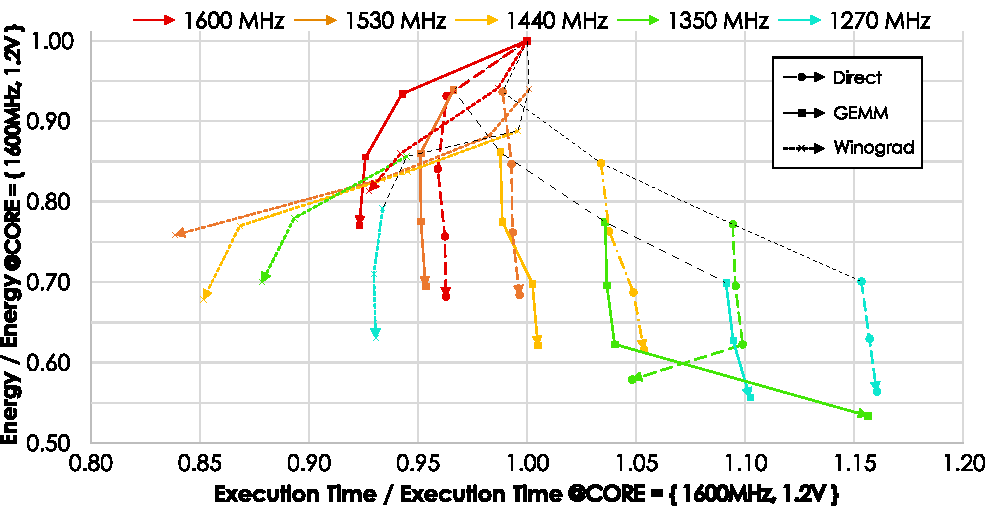
\includegraphics[width=0.47\textwidth]{Figures/Application To Deep Learning/Convolution_Inference_Behaviour.pdf}}
    \subfigure[Training]{\label{fig:Convolution_Backprop_behaviour}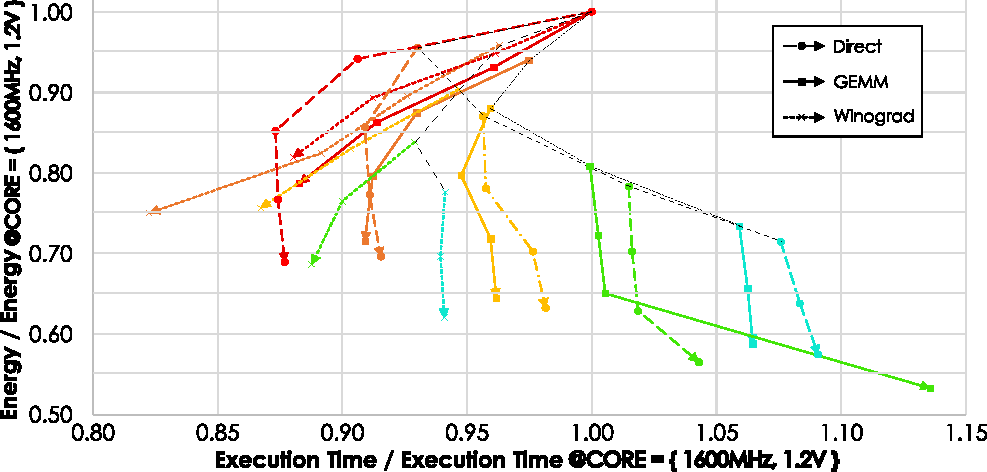
\includegraphics[width=0.47\textwidth]{Figures/Application To Deep Learning/Convolution_Backprop_Behaviour.pdf}}
  \end{subfigmatrix}
  \caption{Core domain - Convolution Layer normalized energy and performance chart to non-conventional V-F configurations.}
  \label{fig:Convolution_behaviour}
\end{figure}

The \acrshort{edp} charts, depicted in Figure~\ref{fig:Convolution_EDP}, indicate that the most energy-efficient configuration for the three algorithms is at the lowest frequencies and maximum undervoltage possible. At these configurations, although the execution time is reduced by $16\%$ (for the \textit{Direct} and \textit{GEMM} algorithms), it is still possible to achieve a reduction in energy consumption of up to $46\%$. The use of the most efficient configuration for the \textit{Winograd} algorithm improves both the execution time and the energy by $15\%$ and $32\%$, respectively.

\begin{figure}[htbp]
    \centering
        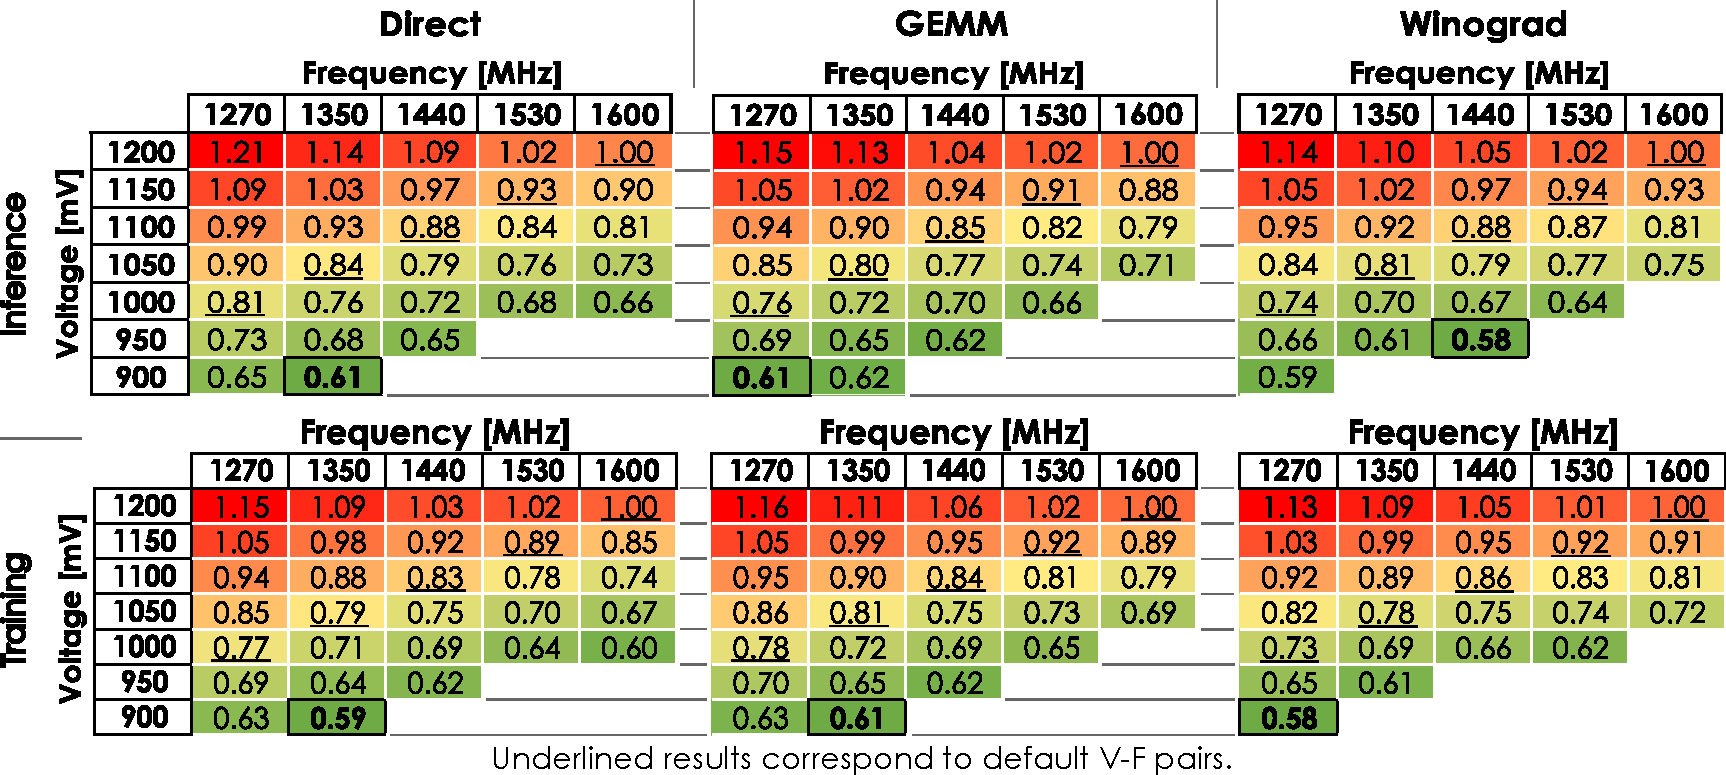
\includegraphics[width=0.9\textwidth]{Figures/Application To Deep Learning/Convolution_EDP.pdf}
        \caption{Core Domain - Convolution Layer - Obtained normalized Energy-Delay Product heat-map for the three algorithms.}
    \label{fig:Convolution_EDP}
\end{figure}



\subsection{Fully-Connected Layer}


The RocBlas library provides a single API for matrix multiplication, the underlying mathematical operation of the fully connected layer. By analyzing the performance counters and the kernels invoked by the library, it is possible to understand that multiplication is performed in one of two ways, depending on the size of the matrices.
According to the work of Nabavinejad~\cite{dutot_high-performance_2016}, small matrices are first loaded to Cache, and all the operations are performed with the data in this memory component, making the operation compute bounded. For large matrices, the matrix multiplication is split, performing the multiplication in a tilling fashion. In this way, submatrices are first loaded to the local caches, and the corresponding submatrices of the results are produced. When the submatrix is consumed, another pair is loaded, and the process repeats until the full computation is performed. The threshold size of the submatrices corresponds to the size of the L1 Cache. 


\subsubsection{Layer Characterization}

Non-conventional V-F impact the two implementations of the matrix multiplication in different ways. For the small matrices variant, 
since all the necessary data is already available on the local caches before the computations start, 
it is the ALU that will limit the undervoltage. Consequently, it is expected that a valley-like shape is observable in the performance chart after the application of frequency scaling (see section~\ref{sec:MAC_behaviour}). On the other hand, for large matrix sizes, the cache will be stressed the most, with constant requests on the DRAM-Cache controller limiting the undervoltage. Consequently, the results will be similar to those that were observed in section~\ref{sec:cache_guardband} and \ref{sec:cache_sm__behaviour}. Figure~\ref{fig:MatrixMult_guardband} illustrates the results of the conducted experiment procedure and confirms the prediction: for small matrix sizes, it is possible to perform a higher degree of undervoltage. 


\begin{figure}[htbp]
    \centering
        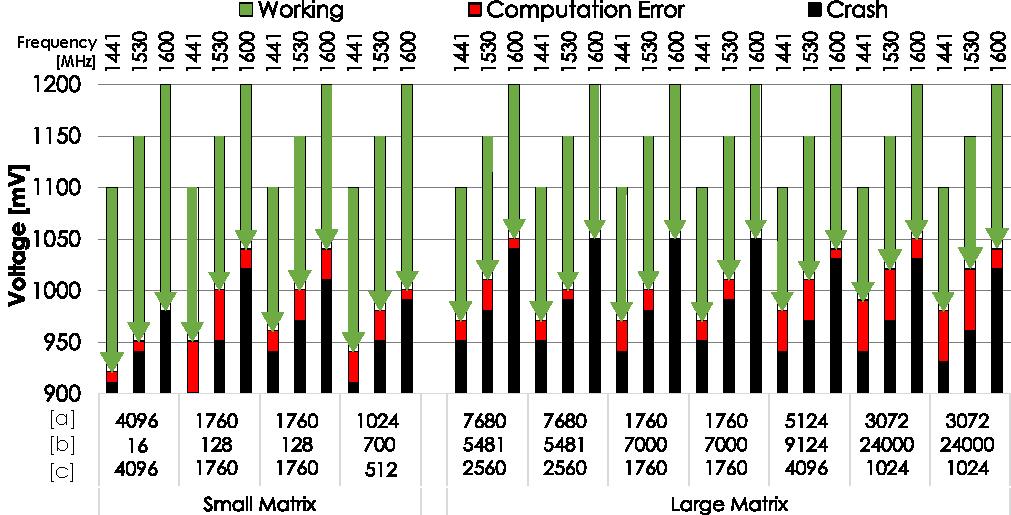
\includegraphics[width=0.65\textwidth]{Figures/Application To Deep Learning/MatrixMul_guardband.pdf}
        \caption{Core Domain - Fully-Connected Layer - Usable GPU core voltage range. $[a]$, $[b]$ and $[c]$ values represent matrix sizes (example $A_{a \times b} \cdot B_{b \times c}$).}
    \label{fig:MatrixMult_guardband}
\end{figure}


From the observation of the results presented in Figures~\ref{fig:MatrixMult_behaviour} and \ref{fig:MatrixMult_EDP} it is possible to conclude that an improvement in the execution time and energy consumption can be achieved for both types of computations. The EDP chart indicates the same energy efficiency configuration for both cases, which results in an average reduction of $52\%$ in energy consumption and $8\%$ of improvement of the execution time.


\begin{figure}[htbp]
    \centering
        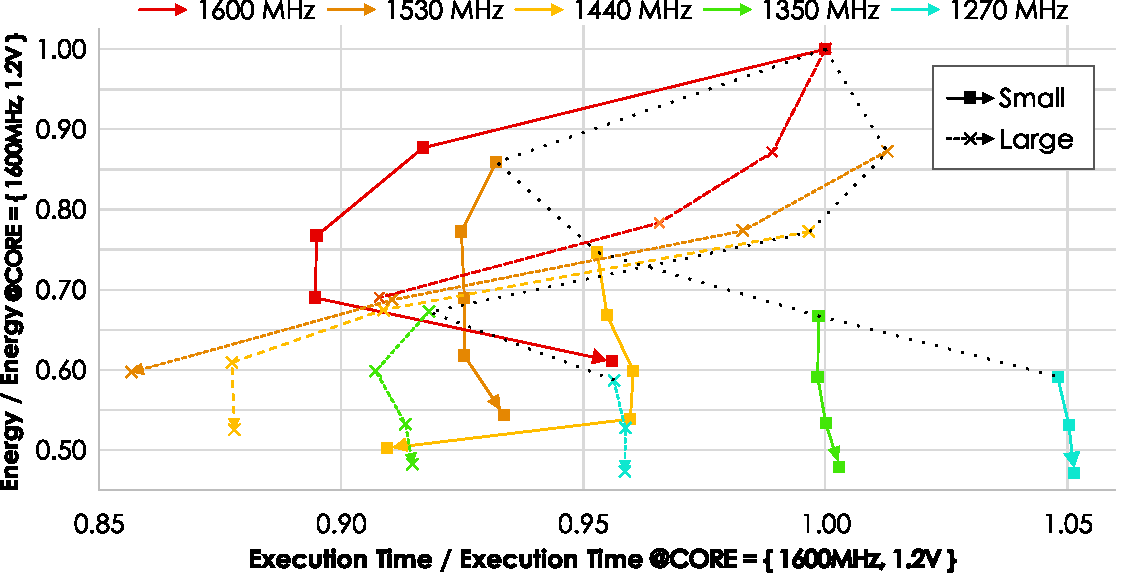
\includegraphics[width=0.65\textwidth]{Figures/Application To Deep Learning/MatrixMul_behaviour.pdf}
        \caption{Core Domain - Fully-Connected Layer normalized energy and performance chart to non-conventional V-F configurations..}
    \label{fig:MatrixMult_behaviour}
\end{figure}





\begin{figure}[htbp]
    \centering
        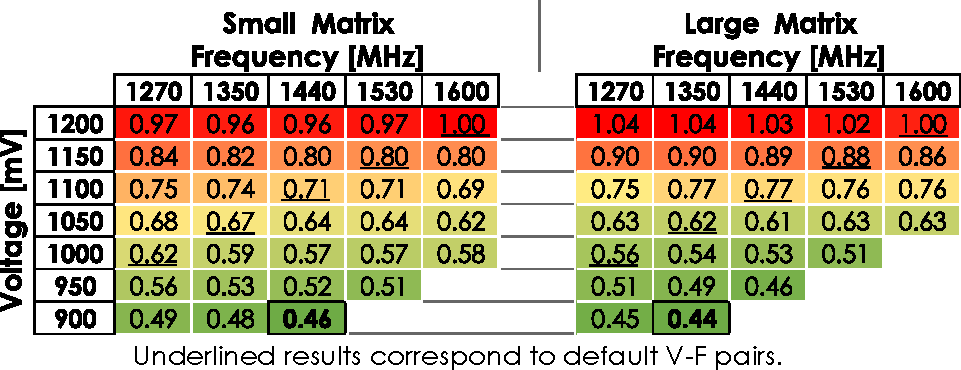
\includegraphics[width=0.65\textwidth]{Figures/Application To Deep Learning/MatrixMul_EDP.pdf}
        \caption{Core Domain - Fully-Connected Layer - Obtained normalized Energy-Delay Product heat-map.}
    \label{fig:MatrixMult_EDP}
\end{figure}

\subsection{Error Analysis}

To evaluate the occurrence of computation errors due to the utilization of non-conventional V-F scaling, each benchmark was executed with the default "automatic" parameterization and with the conventional V-F pair under testing with the same input data. A \textit{warmup\_kernel} was also executed before each of these two runs, to fill the cache with random data. 


For the error analysis of the \acrshort{cnn} layers, a different error metric was adopted due to the utilization of software libraries (versus custom kernels) operating over floating-point numbers (as before, generated from an uniform distribution in the interval $[0.1~;~1]$ to ensure that operations are never applied to numbers with significantly different exponent values). These libraries can launch the kernels in a different order, changing the order of operations, with a possible impact in the final result. In fact, by conducting experiments on the default voltage, it was observed that the kernel execution order resulted in a relative output difference not greater than $10^{-6}$. In accordance, a computation error was asserted whenever the relative difference in each position of the output vectors was greater than or equal to  $10^{-5}$.

\subsubsection{Convolution Layer}

Figure~\ref{fig:Convolution_errors} depicts the distribution of the output results of the convolution layer for the three considered convolution algorithms (at both inference and training phases) for the minimum usable voltage values (i.e., before \acrshort{gpu} crash) across all considered core frequency values. The obtained results emphasize the little effect of the applied undervoltage on the computed values. Most of the output results are still almost entirely accurate, and only a small portion of the results present deviations. In fact, it should be emphasized that not only is the fraction of non-accurate results very small, but the normalized relative error of those non-accurate results has a shallow magnitude. A particular observation is worth noting about the results of the inference phase with the \textit{GEMM} algorithm. Although the amount of non-accurate results is greater than in the other configurations, the normalized relative error's magnitude is much smaller.

\begin{figure}[htbp]
    \centering
        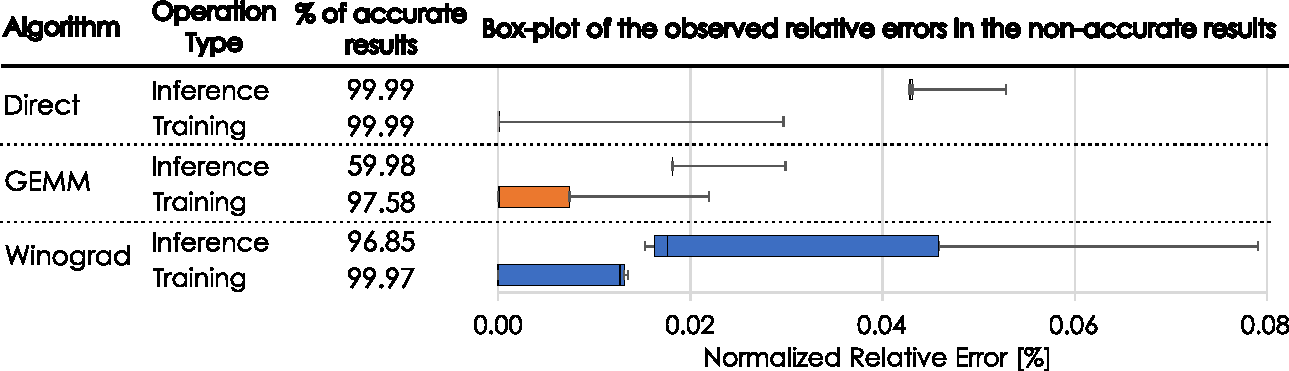
\includegraphics[width=0.8\textwidth]{Figures/Application To Deep Learning/Convolution_Error_Distribution.pdf}
        \caption{Convolution Layer - Average percentage of accurate results and relative error distribution of non-accurate outputs for the minimum usable core voltage across all considered core frequency values.}
    \label{fig:Convolution_errors}
\end{figure}



\subsubsection{Fully Connected Layer}

Figure~\ref{fig:MatrixMult_errors} represents the same error evaluation for the Fully Connected Layer, for both small and large matrices. Even at these extreme configurations, it is observed that most results are still computed with full accuracy (98\% of the cases), with a normalized relative error as low as $1.37\times10^{-3}$ (on the remaining $2$\% of the cases).

\begin{figure}[htbp]
    \centering
        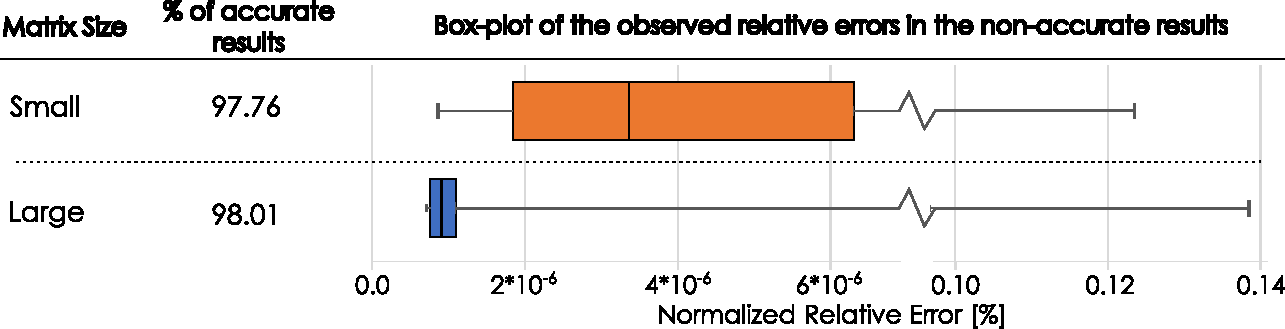
\includegraphics[width=0.8\textwidth]{Figures/Application To Deep Learning/MatrixMul_Error_Distribution.pdf}
        \caption{Fully Connected Layer- Average percentage of accurate results and relative error distribution of non-accurate outputs for the minimum usable core voltage across all considered core frequency values.}
    \label{fig:MatrixMult_errors}
\end{figure}

Hence, the obtained results demonstrate that the amount of error introduced by these lowest voltages before crash conditions, on the two most important layers, are cooped with both \acrshort{dnn} training and inference, demonstrating the ample viability of this approach.


%%%%%%%%%%%%%%%%%%%%%%%%%%%%%%%%%%%%%%%%%%%%%%%%%%%%%%%%%%%%%%%%%%%%%%%%
\section{CNN training and inference with non-conventional V-F}
\label{section:enhanced}

The preliminary assessment of the main \acrshort{cnn} primitives, presented in the previous sections, exhibits the same behavior of the primitive operations analysis, performed in Chapter~\ref{chapter:gpu_char}. From the obtained results, it can be concluded that it is possible to safely undervolt the \acrshort{gpu} of the two main \acrshort{cnn} primitives without compromising the accuracy and with relevant energy and performance gains. In accordance, the logical next step is to adapt the optimization mechanism described in Chapter~\ref{chapter:mech} to the training procedure of complete state-of-the-art \acrshort{cnn}s.


This section starts by presenting the usability of non-conventional V-F on the complete training of \acrshort{cnn}s, followed by a description of how the optimization mechanism was adapted to achieve the same energy efficiency gains automatically.

\subsection{Feasibility Assessment}
\label{sec:fea_ass}
The results that were obtained in the previous section evidence that the small number and relative amount of computation errors introduced by these near threshold conditions is well cooped with the operations that are conducted in \acrshort{dnn} layers. However, the same evaluation urged to be done for the whole network.


Following the same methodology as before, an exploration of decoupled frequency and voltage variations was performed for the training + inference and inference phase of four complete well-know \acrshort{cnn} models. The tested models are LeNet~\cite{lecun_gradient-based_1998}, VGG11~\cite{simonyan_very_2015}, AlexNet~\cite{krizhevsky_imagenet_2012} and WideResNet~\cite{zagoruyko_wide_2017}, corresponding to increasing model sizes, complexity, and characteristics. This feasibility assessment will prove that the considered voltage and frequency scaling is allowed by the algorithms under execution, both with negligent impacts on the models' final training accuracy and with considerable energy-efficiency improvements. To guarantee that the changing V-F is the only source of the observed variation, in all tests, the networks' weights are initialized with the same value.


\subsubsection{Training and Inference}

Table~\ref{tab:trainingAcc} presents the median classification accuracy over ten training runs of the considered networks after applying four different undervoltage levels. The obtained results demonstrate that, when compared with the default setup (i.e., undervolt = 0), the introduced computation errors do not induce any significant change in the network's final training accuracy. 
In more detail, Figure~\ref{fig:CNN_loss}, presents the behavior of the loss and model accuracy of each network, measured on the test set over the training session on all the tested V-F pairs. It is possible to observe that the two metrics' progress is, within small variations, the same for all tested V-F configurations.

\begin{table}[htb]
    \centering
   
    \label{tab:trainingAcc}
    \begin{tabular}{rcccc}
        \multicolumn{1}{l}{{\textbf{Amount of undervolt {[}mV{]}}}} &
          \textbf{AlexNet {[}\%{]}} &
          \textbf{LeNet {[}\%{]}} &
          \textbf{VGG11 {[}\%{]}} &
          \textbf{WideResNet {[}\%{]}} \\ \hline
        \textbf{0}   & 76.59 & 59.84 & 86.14 & 80.32 \\
        \textbf{50}  & 76.48 & 60.08 & 86.14 & 80.39 \\
        \textbf{100} & 76.60 & 59.94 & 86.04 & 80.23 \\
        \textbf{150} & 76.61 & 60.12 & 86.39 & 80.08 \\ \hline
        \multicolumn{1}{l}{{\textbf{Number of trained epochs}}} &
          50 &
          100 &
          30 &
          30
    \end{tabular}%
     \caption{Comparing CNN training test set accuracy with the application of different undervoltage levels.}
\end{table}

\begin{figure}[htb]
    \centering
        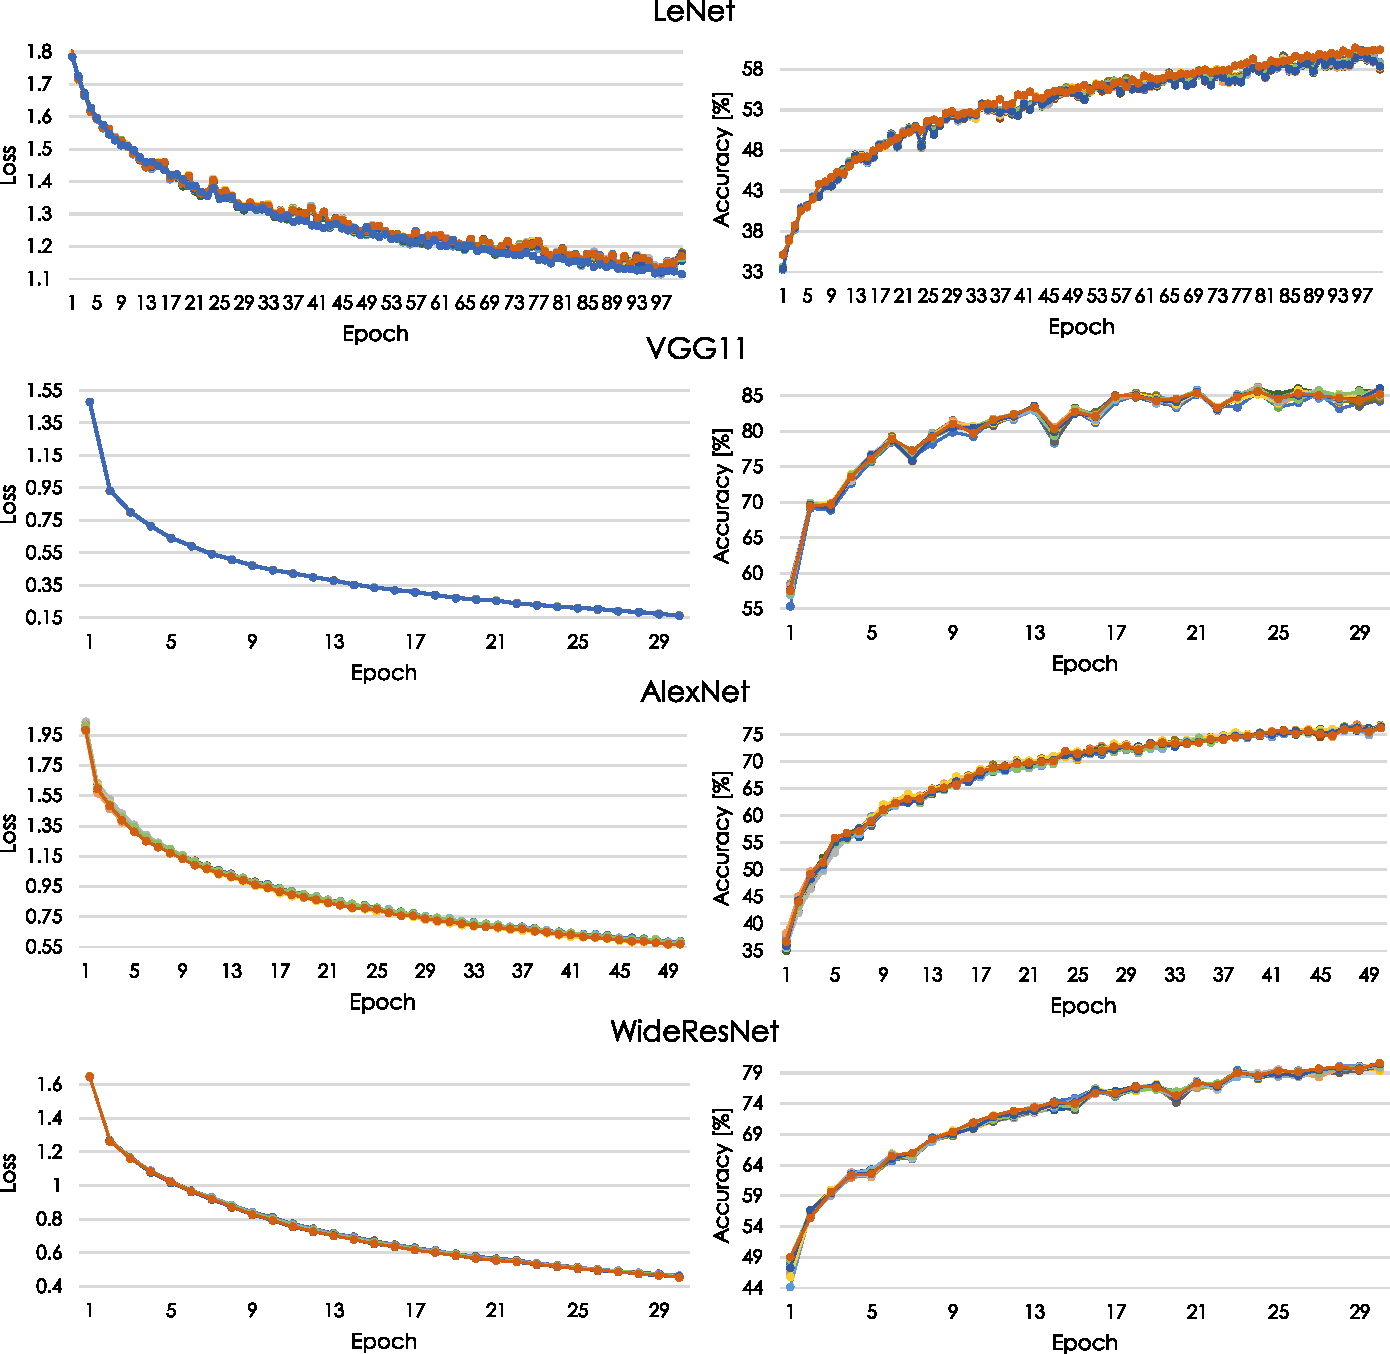
\includegraphics[width=\textwidth]{Figures/Application To Deep Learning/CNN_loss_acc.pdf}
        \caption{Core domain - CNN models - superposition of all V-F configuration test set loss and model accuracy.}
    \label{fig:CNN_loss}
\end{figure}

Figures~\ref{fig:CNN_Behaviour_training_inf} and \ref{fig:CNN_EDP_training_inf} depict the energy performance charts and \acrshort{edp} results for the conducted V-F exploration. Of significant importance is the comparison of the automatic \acrshort{dvfs} system versus the non-conventional V-F configurations, represented as a black dot Figure~\ref{fig:CNN_Behaviour_training_inf}. For this configuration, the training procedure was executed, while allowing the \acrshort{dvfs} system to vary the current V-F pair and adjust all parameters automatically. In neither of the four tested models, the automatic system can achieve the best performance or energy consumption, demonstrating the analysis provided in Chapter~\ref{chapter:background}, that the automatic \acrshort{dvfs} systems of \acrshort{gpu}s are not able to take full advantage of the hardware. 

In particular, the default V-F pairs are able to produce either the lowest energy consumption or the highest performance. 
The main benefit of exploring non-conventional V-F is allowing for higher or even the highest frequency (maximizing performance) while having similar energy consumption to using the lower frequency/energy savings performance levels.
Overall, these new configurations decrease the \acrshort{edp} of the training sessions the most, as depicted in Figure~\ref{fig:CNN_EDP_training_inf}.



\begin{figure}[!htb]
    \centering
        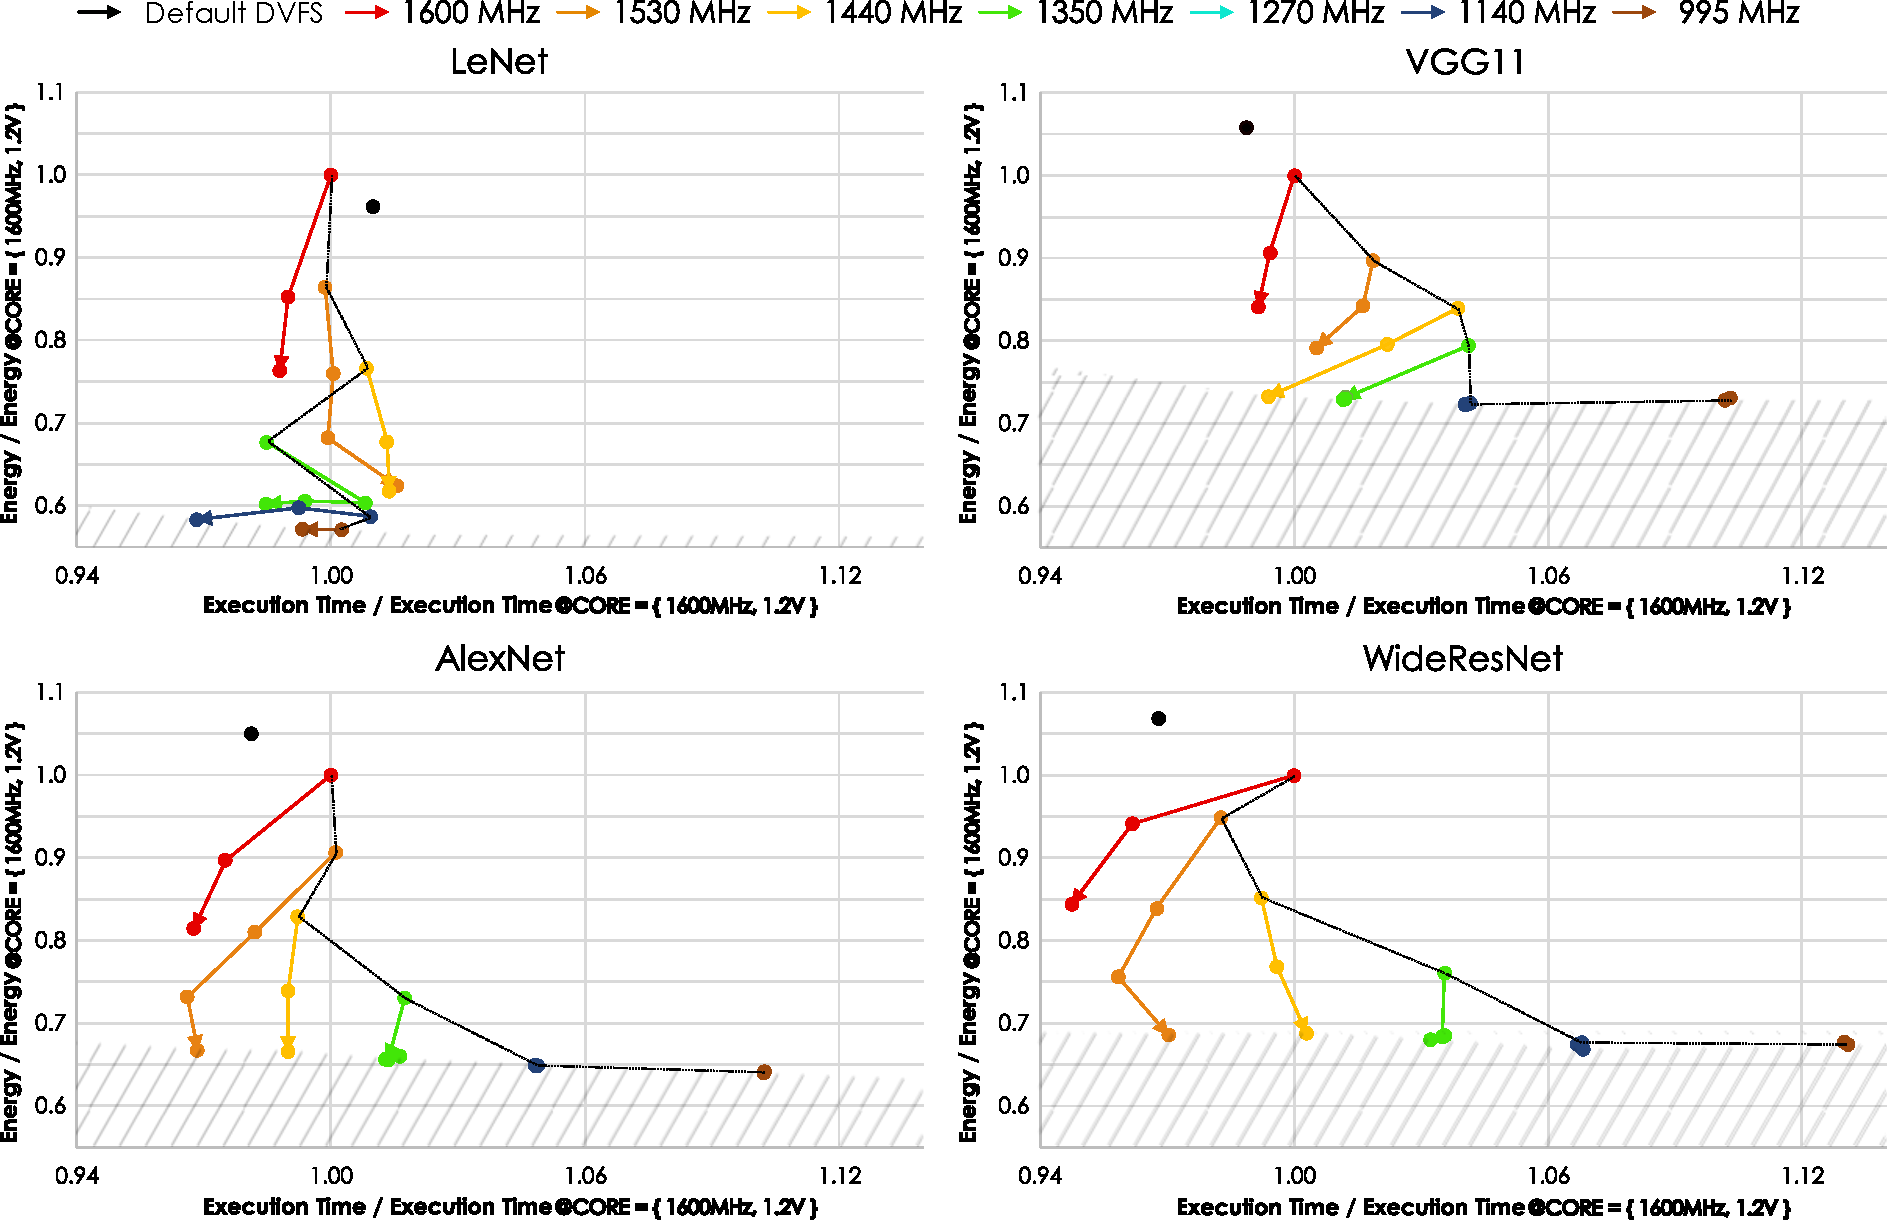
\includegraphics[width=0.85\textwidth]{Figures/Application To Deep Learning/CNN_behaviour.pdf}
        \caption{Core domain - CNN models - Normalized energy consumption and execution time for training + inference. The dashed line connects the default V-F pairs, and the diagonal striped pattern indicates the plateau of minimum energy consumption.}
    \label{fig:CNN_Behaviour_training_inf}
\end{figure}

\begin{figure}[!htb]
    \centering
        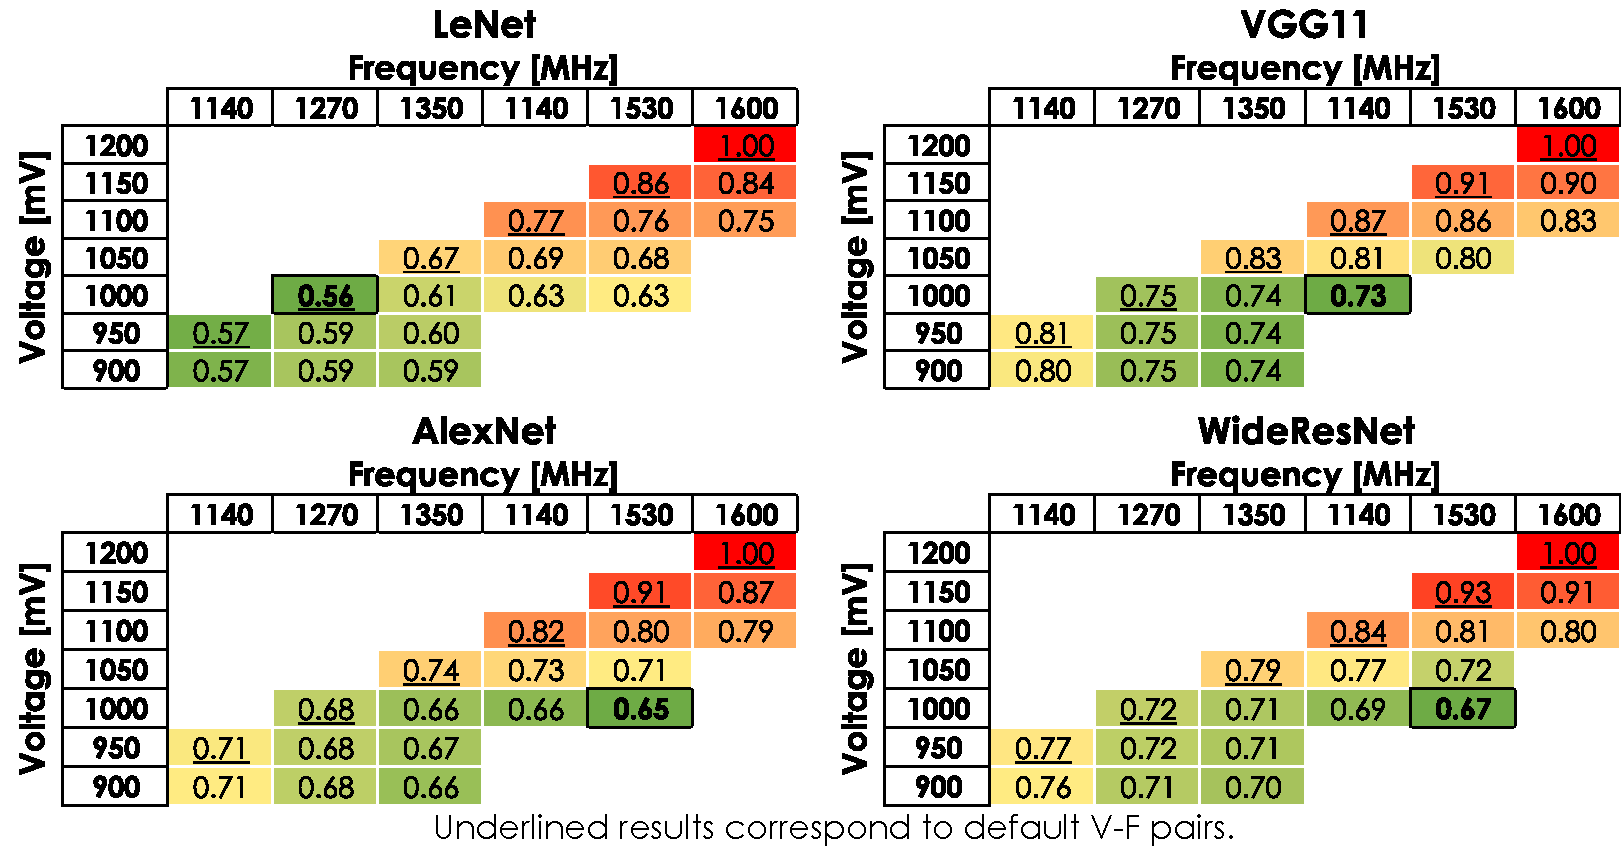
\includegraphics[width=0.8\textwidth]{Figures/Application To Deep Learning/CNN_EDP.pdf}
        \caption{Core domain - CNN models - Obtained normalized Energy-Delay Product (EDP) for training + inference.}
    \label{fig:CNN_EDP_training_inf}
\end{figure}

Table~\ref{tab:trainingMetricsResults} emphasizes and summarizes the main achievements when running the \acrshort{cnn} training under non-conventional V-F. It compares the \acrshort{cnn} execution at the default V-F setup, with the results obtained with frequency scaling using the default voltage values to non-conventional V-F. It considers two configurations: (i) at the highest frequency, and (ii) at minimum EDP. As it can be observed, by exploring non-conventional V-F, it is possible to significantly improve all three metrics (energy, training time, and EDP) without compromising the resulting accuracy of the whole \acrshort{cnn}. 

\begin{table}[htbp]
    \centering
    \label{tab:trainingMetricsResults}
    \begin{tabular}{llcccc}
        &  &  \multicolumn{4}{c}{\textbf{Improvement {\it vs} default V-F}} \\ 
        \cline{3-6} 
        \bf Metric &  \bf Selected configuration &    \textbf{AlexNet} &  \textbf{LeNet} &  \textbf{VGG11} &  \textbf{WideResNet} \\ \hline
        \textbf{Energy}        & At highest frequency & 24\% & 20\% & 22\% & 23\% \\
        \textbf{}              & At best EDP          & 38\% & 38\% & 33\% & 38\% \\\hline
        \textbf{Training time} & At highest frequency & 1\%  & 2\%  & 0\%  & 6\%  \\
        \textbf{}              & At best EDP          & 3\%  & -3\% & -2\% & 0\% \\\hline
        \textbf{EDP}           & At highest frequency & 21\% & 22\% & 22\% & 23\% \\
        \textbf{}              & At best EDP          & 38\% & 41\% & 32\% & 36\% \\ \hline
        
        &  &\multicolumn{4}{c}{\textbf{Improvement {\it vs} F scaling with default V-F pairs}} \\ \hline
        \textbf{Energy}        &At best EDP&  -2\% & 0\% & -1\% & -2\% \\\hline
        \textbf{Training time} &At best EDP&  8\%  & 0\%  & 6\%  & 10\%  \\\hline
        \textbf{EDP}           &At best EDP&  3\% & 0\% & 3\% & 6\% \\ \hline
        \multicolumn{6}{c}{a positive value indicates an improvement vs the default V-F configuration of the GPU.} \\
    \end{tabular}%
    \caption{Evaluation of performance, energy, and EDP when applying non-conventional DVFS in the training of neural networks.}
\end{table}

\newpage

\subsubsection{Inference}

The inference of the same \acrshort{cnn} models was also tested independently. This test tries to understand if the same V-F configuration should be used for the algorithm's inference part. Figure~\ref{fig:CNN_EDP_inf} exhibits the \acrshort{edp} values for the V-F exploration of the four \acrshort{cnn} models. By comparing the \acrshort{edp} heat-maps of the training + inference (Figure~\ref{fig:CNN_EDP_training_inf}) versus the heat-maps of the inference (Figure~\ref{fig:CNN_EDP_inf}), it was observed that the configuration that minimizes the \acrshort{edp}, and so, maximizes the energy-efficiency, only matches on the VGG11 model. However, it should be noted that the same model's heat-maps present an approximate distribution, with the global minimum being around the same V-F configurations for training and inference.

\begin{figure}[htb]
    \centering
        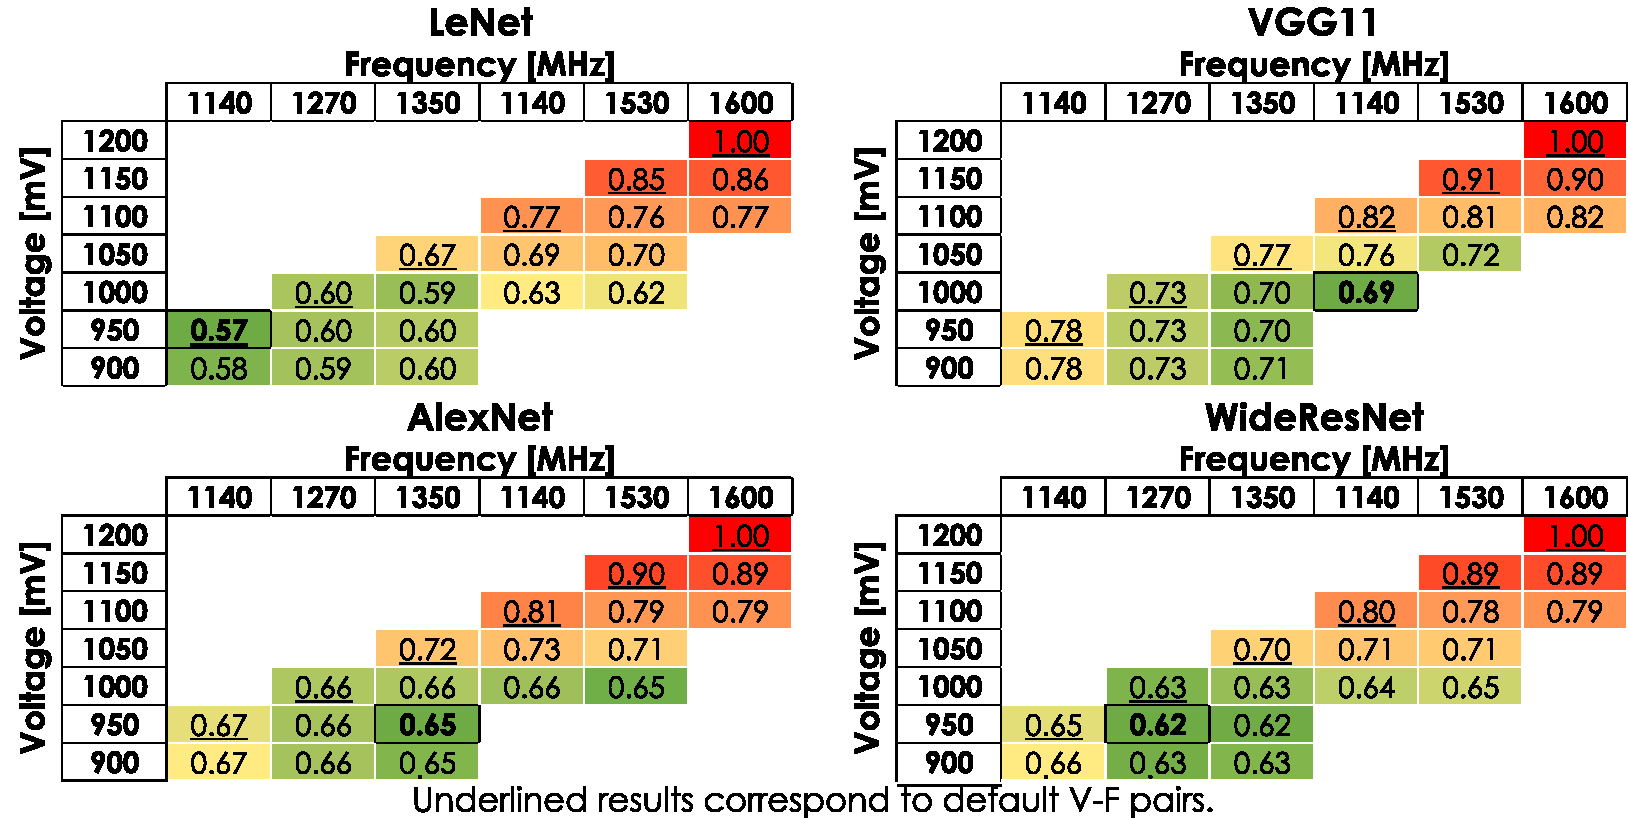
\includegraphics[width=0.8\textwidth]{Figures/Application To Deep Learning/CNN_EDP_inf.pdf}
        \caption{Core domain - CNN models - Obtained normalized Energy-Delay Product (EDP) for inference phase.}
    \label{fig:CNN_EDP_inf}
\end{figure}

\subsection{Optimization algorithm adaptation to CNN training}

To benefit from automatically adjusting the V-F configuration to \acrshort{cnn} training, the developed V-F optimization mechanism, presented in the previous Chapter, was applied to the training procedure.

As the block diagram of Figure~\ref{fig:opt_mech} presents, the V-F optimization mechanism is composed of three stages, \textit{Analysis of user input and test DVFS information}, \textit{Establishment of baseline measurement} and \textit{Optimization Algorithm Execution}. The present subsection indicates how each stage was adapted to the \acrshort{cnn} training procedure and, in specific, in which way the \textit{Online Monitorization} is performed on this application. It is first described the last stage of the Optimization Algorithm Execution - \textit{Optimization Algorithm Execution}, because the way it is implemented conditioned how the two other stages were adapted to this application. Similarly to the example given in Chapter 4, the chosen optimization metric was the energy-efficiency computed as the \acrshort{edp}. 


\subsubsection{Optimization Algorithm Execution}

Chapter 4 described that on the Optimization Algorithm Execution phase of the V-F Optimization Mechanism, the user application is executed on both stages of that phase. In this case, the total number of training epochs would be split by the \textit{Space Exploration} and \textit{Fine-Tunning} stages. However, it was observed that the inference \acrshort{edp} heat-map (see Figure~\ref{fig:CNN_EDP_inf}) presents a similar shape to the training + inference \acrshort{edp} heat-map (see Figure~\ref{fig:CNN_EDP_training_inf}), with both having the $min(EDP)$ at the same or near the same V-F pair.
Nonetheless, executing one inference epoch is significantly faster than running one training + inference epoch. This observation presented the idea of instead of executing the \acrshort{cnn} training procedure in the two Optimization Algorithm Execution stages, execute instead just the inference on the \textit{Space Exploration} phase. With this change, at the cost of introducing an overhead to the training procedure since for the first \textit{Space Exploration Steps}, the \acrshort{cnn} model is not being trained, it is possible to complete this stage faster than running the training + inference in each epoch.
Considering that it is on the \textit{Space Exploration} stage that the less energy-efficient configurations are tested, it is possible to spend less time testing them and so, reduce the total energy consumption to complete this stage. 
By doing so, the training procedure of the \acrshort{cnn} model starts with a configuration that is better suited for it, with improved energy-efficiency. 

Figure~\ref{fig:comp} graphically exemplifies the power consumption overtime of the first ten training epochs of a \acrshort{cnn} model to compare the proposed implementation versus the one where the training procedure is executed on both stages of the \textit{Optimization Algorithm Execution}. Rendered in green is the case that was implemented, where ten \textit{Space Exploration Steps} are performed executing just the inference, and after it, on the \textit{Fine Tuning} stage, the \acrshort{cnn} training procedure starts. Represented in orange is the case where the \acrshort{cnn} training procedure starts at the \textit{Space Exploration} stage, executing in each epoch one training + inference pass. The figure exemplifies that at the end of the \textit{Space Exploration} stage, the same power consumption and execution time (length of the epoch 9 in orange and epoch 0 in green) is achieved to execute a training + inference epoch, so the correspondent \acrshort{edp} value is the same in both cases. Overall, this chart graphically represents the result obtained when adapting the V-F optimization mechanism to the training procedure of \acrshort{cnn} models. The introduced overhead created by not starting the \acrshort{cnn} training procedure at the beginning of the Optimization Algorithm Execution phase is compensated for more quickly finding a more energy-efficient V-F configuration running just the inference of the \acrshort{cnn} model.

\begin{figure}[htb]
    \centering
        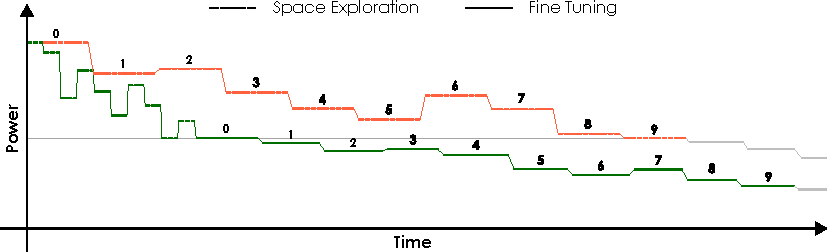
\includegraphics[width=0.95\textwidth]{Figures/Application To Deep Learning/comparacao.pdf}
        \caption{Graphical representation of the power consumption overtime of the first ten training epochs of a \acrshort{cnn} model. The orange line represents the case where the training procedure is started at the Space Exploration stage, and the green line represents the case where the training procedure is only started on the Fine-Tuning stage.}
    \label{fig:comp}
\end{figure}




\subsubsection{Analysis of user input and test DVFS information}

To set the usable execution space for the \acrshort{cnn} training and execution, both the results of the \acrshort{gpu} characterization (presented in Chapter 3) and the specific results of the preliminary assessment performed in this chapter (see Section~\ref{section:baseline}) were used. Figure~\ref{fig:ues} presents the usable execution space for the Vega 10 \acrshort{gpu}, optimized for  \acrshort{cnn} training and execution.

\begin{figure}[htb]
    \centering
        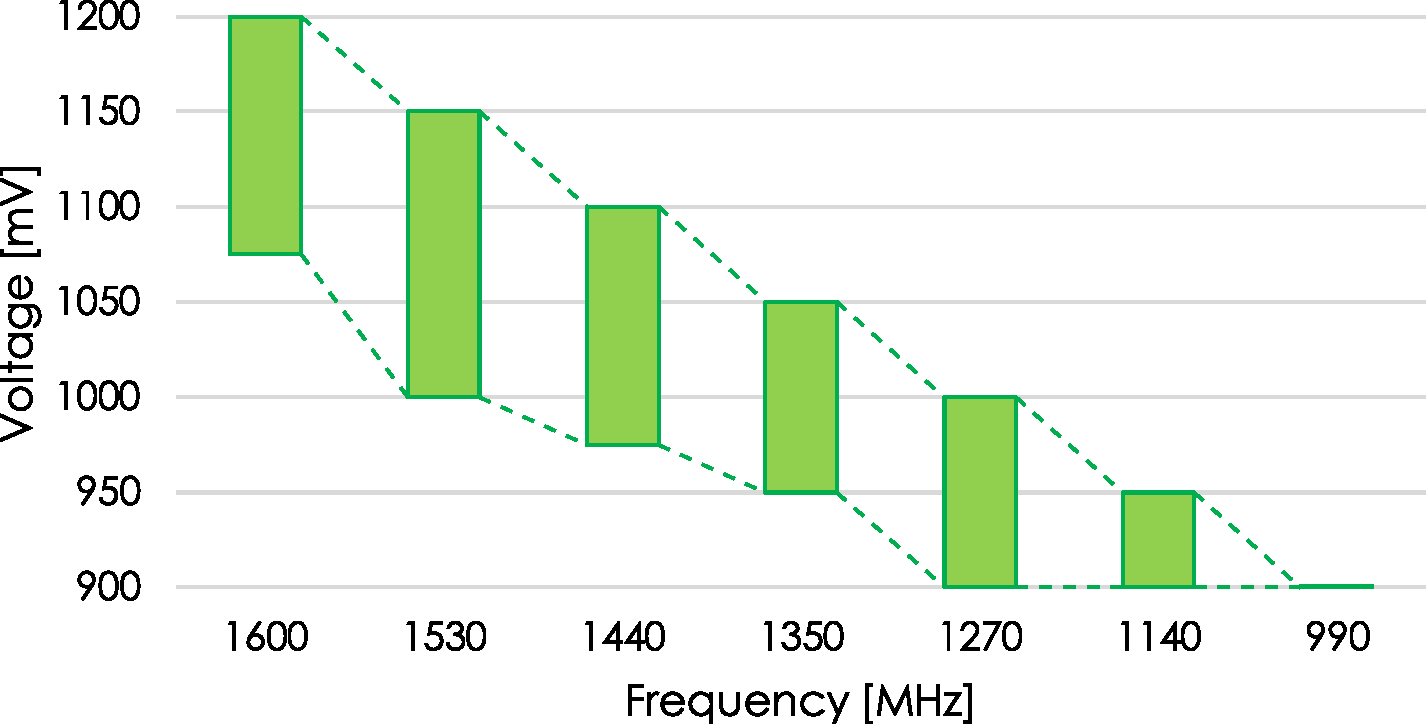
\includegraphics[width=0.6\textwidth]{Figures/Application To Deep Learning/UES.pdf}
        \caption{Usable Execution Space for the Vega 10 \acrshort{gpu}.}
    \label{fig:ues}
\end{figure}



For the first stage of the Optimization Algorithm Execution (\textit{Space Exploration}), only the green bars that correspond to tested frequencies are considered. However, for the second stage of the Optimization Algorithm Execution (\textit{Fine-Tuning}), the area between the dashed lines, corresponding to the linear regression between the margins of two adjacent frequencies, is also regarded as valid V-F configurations.

\subsubsection{Establishment of baseline measurement}

In accordance with the adaptation of the V-F Optimization Mechanism to the \acrshort{cnn} training procedure described above, two individualized baseline measurements are taken, the first covering one inference epoch and the second containing one training + inference epoch. The inference baseline is used on the \textit{Space Exploration} stage, where the training + inference baseline is used for the  \textit{Fine Tuning} stage. To proceed with the measurements, the \acrshort{gpu} was set to the highest V-F configuration \{1600MHz; 1.2V\}, and the execution time and energy consumption were measured, computing the \acrshort{edp} by multiplying both results.





% For these two algorithm execution stages, the logical development would be to split the total number of training epochs by the \textit{Space Exploration} and \textit{Fine-Tunning} stages. However, the inference \acrshort{edp} heat-map (see Figure~\ref{fig:CNN_EDP_inf}) present a similar shape to the training + inference \acrshort{edp} heat-map (see Figure~\ref{fig:CNN_EDP_training_inf}) with one additional significant advantage. Performing just the inference is significantly faster than performing one training epoch. So, it was concluded that in a long training session (with a high number of training epochs), if the \textit{Space Exploration} was performed, optimizing just the inference, this process could be done faster than optimizing the training epoch since the training process would already start with a more energy-efficient V-F configuration. This would offset the initial \textit{Space Exploration} stage, where the algorithm to be optimized is not already being executed.

% The decision was then to execute inference epochs on the \textit{Space Exploration} stage.


% \subsubsection{Algorithm Execution - Fine-tuning}

% For the \textit{Fine-Tunning} stage, the \acrshort{cnn} training proceed as usual. In this stage, the optimization mechanism tries to explore the in-between tested frequencies and voltages to achieve the V-F configuration that results in the most energy-efficiency possible.  

\subsubsection{Online Monitorization}

The considered output validity metrics adopted in the optimization mechanism are the loss function value and the network weights' value. If any of these values becomes not a number (NaN), the output is considered invalid. NaN's appearance in these two values is attributed to computational errors that may occur when the used voltage is near $V_{min}$. To mitigate or at least reduce the computaional error, the voltage value is increased by 10 mV, decreasing the amount of applied undervoltage.



\subsection{Experimental Results}

The four different \acrshort{cnn} architectures were tested under the V-F Optimization Mechanism, with each model being tested 10 times. It was allowed 20 \textit{Space Exploration} epochs, value obtained by measuring how many epochs on average does the algorithm take to achieve a good V-F configuration across the four models. Figure~\ref{fig:3d} presents an example of the V-F configuration and resulting normalized \acrshort{edp} value when applied to the WideResNet model.

\begin{figure}[h]
\centering
    \begin{tikzpicture}
    \begin{axis}
    [  
    width=0.8\linewidth,
    height=0.4\linewidth,
    view={-45}{45},
    xmin=950, xmax=1600,
    ymin=900, ymax=1200,
    zmin=0.5, zmax=1,
    ytick={900, 1000, 1100, 1200},
    ztick={0.5, 0.75, 1},
    xlabel={Frequency [MHz]},
	ylabel={Voltage [mV]},
	zlabel={EDP/EDP@CORE=\{1600MHz;1.2V\}},
	label style=sloped,
	%point meta=explicit symbolic,
	nodes near coords
    ]
    \addplot3[ycomb,scatter] file {./3d_data.dat};
    \addplot3[scatter] file {./3d_data.dat};
    \end{axis}

    \end{tikzpicture}
    \caption{WideResNet \textit{Space Exploration} example - normalized \acrshort{edp} values for 20 epochs. Initial value is 1600MHz and 1.2V.}
    \label{fig:3d}
\end{figure}


At the end of the \textit{Space Exploration}, performed with just an inference epoch, the V-F configuration that achieved the lowest \acrshort{edp} value is given for the textit{Fine-Tuning} stage, where the \acrshort{cnn}  training process is executed.

The developed optimization mechanism can achieve an even higher degree of energy-efficiency than the previous sections' results. This comes from the better fine-tuning of frequency and voltage that is performed during the \acrshort{cnn} training. Figure~\ref{fig:Algori_comp} compares the \acrshort{edp} of the default \acrshort{dvfs} system versus the best V-F configuration found on the feasibility assessment, the best found configuration achievable (attained by performing a new training session with the final configuration chosen by optimization algorithm) and training with the optimization algorithm (that encompasses the overhead attained by running the \textit{Space Exploration} with only an inference epoch). Training with the developed mechanism yields a reduction of the \acrshort{edp} of 27\% to 42\% over the default \acrshort{dvfs} system. In two of the cases, the developed mechanism with its optimization overhead is even able to beat the best configuration found in Section~\ref{sec:fea_ass}. This is due to the best possible V-F not being one of the tested frequencies. For the other two cases, the mechanism only falls less than 5\% short compared to the previous results. However, this mechanism able to achieve this acrshort{edp} optimization without any prior testing of the acrshort{cnn} model and while performing the final training procedure.
\begin{figure}[htb]
    \centering
        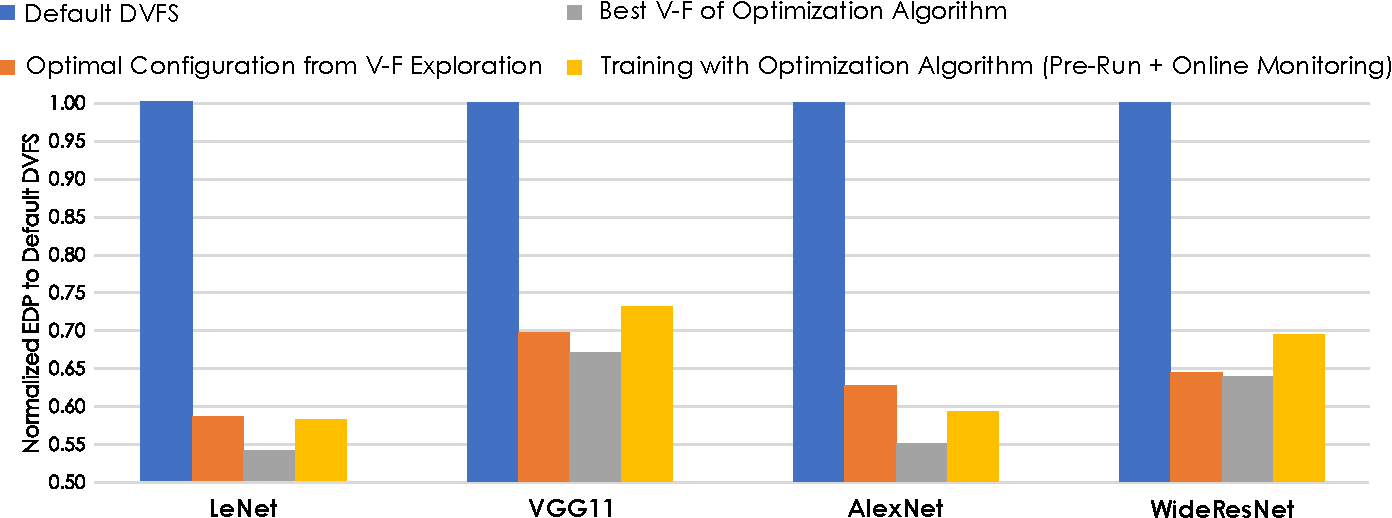
\includegraphics[width=0.95\textwidth]{Figures/Application To Deep Learning/Algorithm_Opt_comp.pdf}
        \caption{Median normalized EDP of default DVFS vs training CNN with V-F optimization model.}
    \label{fig:Algori_comp}
\end{figure}

Table~\ref{tab:bestVF} indicates the mode V-F configuration (configuration that appeared more times) at the end of each algorithm execution stages.

\begin{table}[htb]
    \centering
    \label{tab:bestVF}
    \begin{tabular}{lcccc}
        \multicolumn{1}{r}{{\textbf{Model}}} &  \textbf{LeNet} & \textbf{VGG11} &\textbf{AlexNet} & \textbf{WideResNet} \\ \hline
        \textit{Space Exploration} &  [1140MHz; 0.95V] & [1140MHz; 1.0V] & [1350MHz; 0.95V]  & [1350MHz; 0.9V]\\
        \textit{Fine-Tunning} &  [1230MHz; 0.95V] & [1370MHz; 0.97V] & [1410MHz; 0.98V]  &[1500MHz; 0.99V]\\ \hline
    \end{tabular}%
     \caption{Mode of selected V-F configurations at the end of each optimization stage.}
\end{table}



\section{Summary}

Deep learning and, more specific deep neural networks are a prominent type of algorithm being executed on \acrshort{gpu}s nowadays. These types of algorithms use special mathematical operations (like the convolution) to be able to extract features from the input data. The execution (inference) of these algorithms and, more importantly, the training session can significantly benefit if the energy-efficiency of \acrshort{gpu}s improves.

This chapter combines all the previous knowledge acquired and presented in the previous chapter of the dissertation. It sets the usable execution space of the convolutional neural networks and, it adapts the V-F Optimization Mechanism to the training of this algorithm with excellent results. By characterizing the target \acrshort{gpu} to the target application, it was concluded that the energy efficiency of the training session could be significantly improved, with an \acrshort{edp} reduction of 27\% to 42\% depending on the \acrshort{cnn} model, over the default \acrshort{dvfs} system.
